\documentclass[a4paper]{article}

\usepackage[margin=2.5cm]{geometry}
\usepackage[pdftex]{graphicx}
\usepackage[utf8]{inputenc}
\usepackage[T1]{fontenc}
\usepackage{textcomp}
\usepackage{babel}
\usepackage{amsmath, amssymb}
\usepackage[colorlinks=true,linkcolor=blue]{hyperref}
\usepackage{float}
\usepackage{mathrsfs}
%\usepackage{enumitem}
%% for identity function 1:
\usepackage{bbm}
%%For category theory diagrams:
%\usepackage{tikz-cd}
%%For code (e.g. python) in latex:
%\usepackage{listings}
%
%Usage: 
%\begin{lstlisting}[language=Python]
%\end{lstlisting}

\newcommand{\incfig}[2][1]{%
\def\svgwidth{#1\columnwidth}
\import{./figures/}{#2.pdf_tex}
}


% figure support
\usepackage{import}
\usepackage{xifthen}
\pdfminorversion=7
\usepackage{pdfpages}
\usepackage{transparent}

\pdfsuppresswarningpagegroup=1

\setlength\parindent{0pt}

\newcommand{\qed}{\tag*{$\blacksquare$}}
\newcommand{\qedwhite}{\hfill \ensuremath{\Box}}

%Inequalities
\newcommand{\cycsum}{\sum_{\mathrm{cyc}}}
\newcommand{\symsum}{\sum_{\mathrm{sym}}}
\newcommand{\cycprod}{\prod_{\mathrm{cyc}}}
\newcommand{\symprod}{\prod_{\mathrm{sym}}}

%Linear Algebra

%Redeclaring Span and image
\DeclareMathOperator{\Span}{span}
\DeclareMathOperator{\Ima}{Im}
\DeclareMathOperator{\diag}{diag}
\DeclareMathOperator{\Ker}{Ker}
\DeclareMathOperator{\ob}{ob}


%Row operations
\newcommand{\elem}[1]{% elementary operations
\xrightarrow{\substack{#1}}%
}

\newcommand{\lelem}[1]{% elementary operations (left alignment)
\xrightarrow{\begin{subarray}{l}#1\end{subarray}}%
}

%SS
\DeclareMathOperator{\supp}{supp}
\DeclareMathOperator{\Var}{Var}

%NT
\DeclareMathOperator{\ord}{ord}

%Alg
\DeclareMathOperator{\Rad}{Rad}
\DeclareMathOperator{\Jac}{Jac}

\DeclareMathAlphabet{\pazocal}{OMS}{zplm}{m}{n}
\newcommand{\unif}{\pazocal{U}}

\begin{document}
\textbf{1:} Let $\mathcal{U} = \left\{ X - Z  \colon Z \subset X \text{ is an
algebraic subset} \right\} $.\\
    (a) By the remark on page 6 on lecture note 10, it suffices to check that
    the union of finitely many algebraic sets is an algebraic set, that
    the intersection of an arbitrary collection of algebraic sets is an
    algebraic set, and finally that $\varnothing$ and $X$ are
    in $\mathcal{U}$.\\
    The first two requirements follow from page 7 on lecture note 1, where we
    have that arbitrary intersections of algebraic sets are algebraic sets and
    finite unions of algebraic sets are algebraic sets:\\
    $\bigcap_{i \in  I} V(S_i) = V \left( \bigcup_{i \in  I} S_i \right) $ with
    $I$ arbitrary, and
    $\bigcup_{i =1}^{n} V(S_i) = V\left( S_1 \ldots S_n \right) $.\\
    The last requirement follows since $X = V(0)$ and hence
    $\varnothing = X - X \in \mathcal{U}$. Similarly, 
    $\varnothing = V(1)$, so $X = X - \varnothing \in \mathcal{U}$.\\
    \linebreak
    (b) By the lemma on page 1 of lecture note $9$, we have
    that for any algebraic subset $Z \subset Y$, we have
    $\varphi^{-1}(Z)$ is an algebraic subset of $X$. Equivalently, the
    preimage of any closed subset of $Y$ is a closed subset of $X$ which by the
    remark on page 2 of lecture note 11 is equivalent to $\varphi$ being
    continuous with respect to the Zariski topology on both spaces.\\
    \linebreak
    (c) By Hilbert's basis theorem, there exist $f_1, \ldots, f_n
    \in k\left[ x_1, \ldots, x_n \right] $ such that
    $Z = V\left( f_1, \ldots, f_n \right) = V(f_1)
    \cap \ldots \cap V(f_n)$. The set
    $V(f_i) = \left\{ (x_1, \ldots, x_n) \in \mathbb{A}^{n}  \mid 
    f_i \left( x_1, \ldots, x_n \right) = 0\right\} 
    = f_i^{-1}\left( \left\{ 0 \right\}  \right) $. Considering
    $\mathbb{C}^{n}$ and $k$ with the classical topology and using that
    $f_i$ is a polynomial and thus continuous, we find that since
    $\left\{ 0 \right\} $ is a singleton and thus closed, that
    $f_i^{-1}(\left\{ 0 \right\} )  = V\left( f_i \right) $ is closed in the
    classical topology on $\mathbb{A}^{n} \cong \mathbb{C}^{n}$.\\
    Therefore the Zariski topology is coarser than the classical topology.\\
    \linebreak
    \textbf{2:}\\
    (a) Let $A = \left\{ \left( \sin t, \cos t \right)  \colon t \in \mathbb{R}
    \right\} \subset \mathbb{A}_{\mathbb{C}}^2  $.  We have
    $x^2 + y^2 -1 \in I(A) \subset \mathbb{C} \left[ x,y \right] $, so
    $\overline{A} = V\left( I\left( A \right)  \right) \subset 
    V\left( x^2 + y^2 -1 \right)$.\\
    Now we can note for example that
    $x^2 + y^2 -1 \in \mathbb{C}[y][x]$ is Eisenstein at $(y-1)$ which is
    prime since it is irreducible since it is linear; hence
    $x^2 + y^2 -1$ is irreducible, so $V(x^2 + y^2 -1)$ is irreducible since
    it is infinite, by corollary 1 chapter 1.6, Fulton. Now by corollary 2
    in chapter 1.6, Fulton, we have that any non-empty proper algebraic subset
    of $V\left( x^2 + y^2 -1 \right) $ must be either a finite union of
    points or a finite union of irreducible plane curves.\\
    However,
    if say $\overline{A} = V \left( g_1, \ldots, g_k \right) $, and $V(g)$ for
    $g = g_i$ for some $i \in \left\{ 1,\ldots,k \right\} $,
    is an irreducible plane curve contained in $V(x^2 + y^2 -1)$,
    then
    $(x^2 + y^2 -1) \subset (g)$. And since $x^2 + y^2 -1$ is irreducible, we
    must have that $g$ is either a unit or associated to $x^2 + y^2 -1$.
    If $g$ were unit, then $\overline{A} = V\left( g_1, \ldots, g_k \right) 
    \subset V(g) = \varnothing$, contradiciton. Thus $g$ must be associated to
    $x^2 + y^2 -1$. So $(g) = \left( x^2 + y^2 -1 \right) $. Since $g$ was
    arbitrary of the $g_i$, we get
    $(g_1, \ldots, g_k) =  (x^2 + y^2 -1)$, so
    $\overline{A} = V\left( x^2 + y^2 -1 \right) 
    = \left\{ \left( \sqrt{1 - z^2} , z \right)  \mid z \in \mathbb{C} \right\} 
    \cup \left\{ \left( - \sqrt{1-z^2} ,z \right)  \mid z \in \mathbb{C} \right\} $.\\

    \begin{figure}[H]
        \centering
        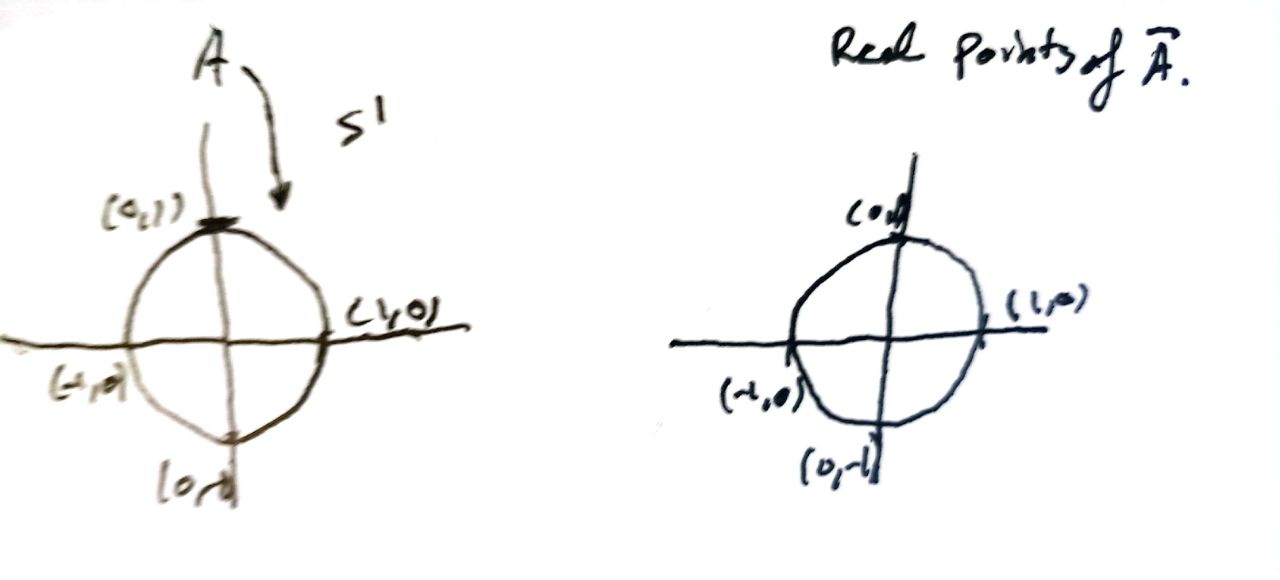
\includegraphics[width=0.8\textwidth]{1.jpg}
        \label{fig:1-jpg}
    \end{figure}

    (b) Let $B = \left\{ \left( x,y,z \right)  \colon z>0 \right\} 
    \subset \mathbb{A}_{\mathbb{R}}^{3}$. We have by the first lemma on lecture
    note 11 that 
    $\overline{B} = V\left( I\left( B \right)  \right) $. Now, assume
    $f \in I(B)$. Then, fixing $x_0, y_0 \in \mathbb{R}$, we have
    a map $\varphi \in k\left[ t \right]  $ by
    $\varphi(t) = f\left( x_0, y_0, t \right) $ which, by assumption, 
    vanishes on $\mathbb{R}_+$. Thus $\mathbb{R}_+ \subset V\left( \varphi
    \right) $, but by problem 1.8 in Fulton, we have that
    the algebraic subsets of $\mathbb{A}^{1} (\mathbb{R})$ are the finite
    subsets, together with $\mathbb{A}^{1} (\mathbb{R})$ itself. Since
    $\mathbb{R}_+$ is infinite, we thus have
    $V(\varphi) = \mathbb{A}^{1}(\mathbb{R})$.\\
    Hence, since $ x_0, y_0$ were arbitrary, we have
    that for any  $x_0, y_0$, $V(\varphi) = \mathbb{A}^{1}(\mathbb{R})$ so
    $$V(f) = \bigcup_{\left( x_0,y_0 \right) \in \mathbb{A}^{2}(\mathbb{R})} 
    \left\{ x_0 \right\} \times \left\{ y_0 \right\} \times 
    V\left( f\left( x_0, y_0, t \right)  \right) 
    = \mathbb{A}^{3}\left( \mathbb{R} \right). $$
 
    Hence $I(B) = (0)$. Thus $V\left( I\left( B \right)  \right) = 
    \mathbb{A}_{\mathbb{R}}^{3}$.



\begin{figure}[H]
    \centering
    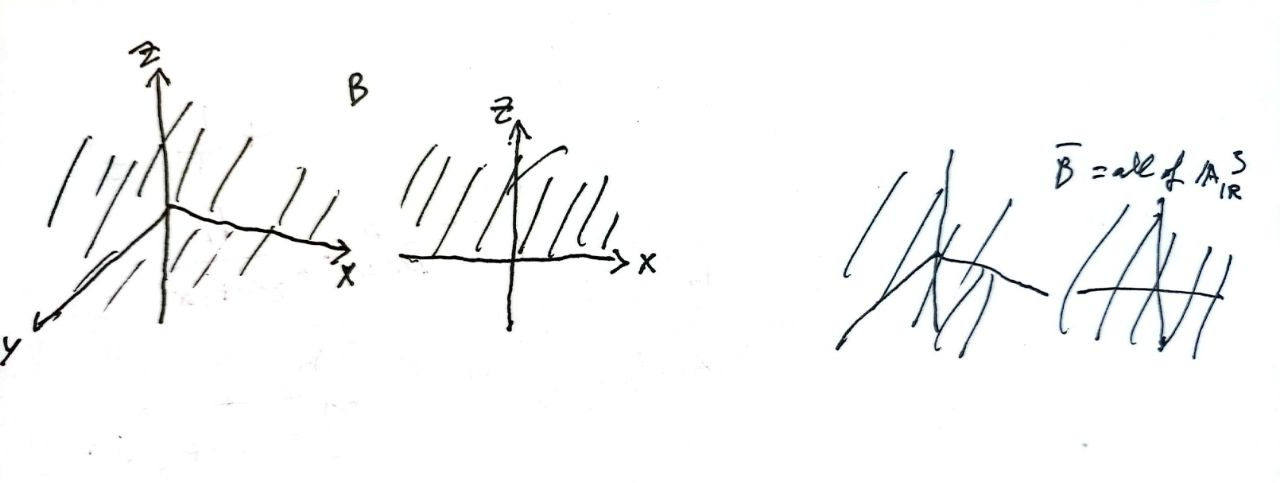
\includegraphics[width=0.8\textwidth]{2.jpg}
    \label{fig:2-jpg}
\end{figure}



    (c) We have
    $C = \left\{ \left( x,y,z \right)  \colon x = y \lor x = z \right\} 
    = \left\{ (x,y,z)  \colon x= y \right\} \cup 
    \left\{ (x,y,z)  \colon x = z \right\} 
    = V(x-y) \cup V\left( x-z \right)
    = V\left( (x-y)(x-z) \right) $.\\
    Now, since the closure of $C$ is the smallest algebraic
    subset containing $C$, and $C$ itself is an algebraic subset, we have
    $\overline{C} = C$.
\begin{figure}[H]
    \centering
    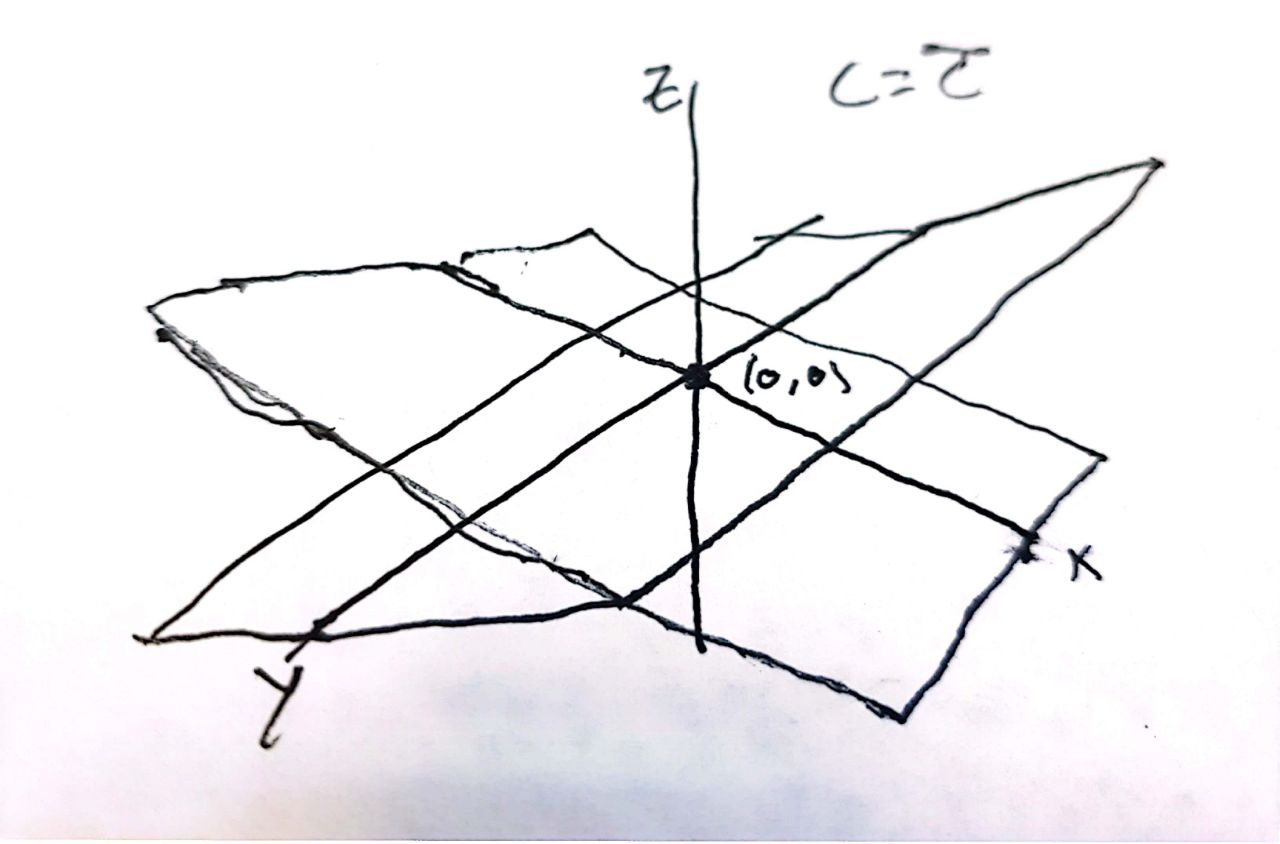
\includegraphics[width=0.8\textwidth]{3.jpg}
    \caption{This is the union of the two plane $x=y$ and $x=z$.}
    \label{fig:3-jpg}
\end{figure}


\newpage

\textbf{3:}\\
(a) Let $\varphi^{*}  \colon \Gamma(\mathbb{A}^2) = k\left[ u,v \right] 
\to k\left[ x,y \right] = \Gamma\left( \mathbb{A}^2 \right)$ be the pullback.
Then $\varphi^{*}(u) (x,y) = (u) \left( \varphi (x,y) \right) 
= (u) (xy, y) = xy$ and
$\varphi^{*}(v) (x,y) = (v) (\varphi(x,y)) =
(v) \left( xy, y \right) = y$, so
$\varphi^{*} f(u,v) = f(xy, y) $.\\
\linebreak
(b) We have $\varphi$ dominant if and only if $\varphi^{*}$ is injective.
Now $\varphi^{*}$ is a homomorphism and 
$\varphi^{*}(f(u,v)) = 0$ if and only if $f(xy, y) = 0$. Since
$xy$ and $y$ are linearly independent, we have that $\varphi^{*}$ is injective
and hence $\varphi$ is dominant.\\
The image of $\varphi$ is 
$\left\{ (xy, y)  \mid x,y \in k \right\} $.\\
\linebreak
(c) Since $\varphi$ is dominant, $V\left( I\left( \varphi(\mathbb{A}^2) \right)  \right) 
= \mathbb{A}^2$. If $\varphi\left( \mathbb{A}^2 \right) $ where closed, then
$\varphi \left( \mathbb{A}^2 \right) = V\left( I\left( \varphi\left(
\mathbb{A}^2 \right)  \right)  \right) = \mathbb{A}^2$ which is
a contradiction, so
$\varphi\left( \mathbb{A}^2 \right) $ is not closed.\\
Since $\varphi$ is a morphism, it is continuous with respect to the Zariski
topology, so if $\varphi(\mathbb{A}^2)$ were open, its preimage would be open,
however, the preimage $\mathbb{A}^2$ is closed since it is the hypersurface
of the zero function. Thus the image is neither closed nor open in the Zariski
topology.\\
\linebreak
\textbf{4:} \\
(a) Suppose $A$ is dense in $X$ and $\overline{f} \in \Gamma(X)$ is a polynomial functions
such that $\overline{f}(P) = 0$ for all $P \in A$. Then since
$P \in A \subset X$, we have $f(P) = \overline{f}(P) = 0$ for all $P \in A$,
hence
$f \in V(A)$ so $X = I\left( V\left( A \right)  \right) \subset V(f)$ and hence
$X \subset V(f) = V\left( f \right) \cap X = V\left( \overline{f} \right) $, so
$\overline{f} \in I_X (X)$ and thus
$\overline{f} = 0 \in \Gamma(X)$.\\
\linebreak
(b) We have $\varphi  \colon X \to Y$ is dominant if and only if
$I \left( \varphi(X) \right) = I(Y)$ if and only if
$\overline{\varphi(X)} = V\left( I\left( \varphi(X) \right)  \right) 
= V\left( I\left( Y \right)  \right) = Y$ since $Y$ is an algebraic set - where
the first equality follows from the first lemma on lecture note 11. The
second "if" follows from $I\left( V\left( I\left( X \right)  \right)  \right) 
= I(X)$ by (9) in chapter 1.3, Fulton.\\
\linebreak
(c) We claim the intersection of dense subsets is not always dense. Take
for example $X = \mathbb{R}$. Then $A = \mathbb{Q} \subset \mathbb{R}$ and
$B = \mathbb{R} - \mathbb{Q}$ are both dense subsets. However,
$A \cap B = \varnothing$ which is not dense in $\mathbb{R}$.\\
\linebreak
(d) Let $X$ be an irreducible algebraic set and $U \subset X$ a non-empty open
subset. We claim that
$X = \left( X-U \right) \cup \overline{U}$.\\
\textit{Proof:} Let $x \in X$. If $x \not\in X-U$ then $x \in U$ and hence
$x \in \overline{U}$ since $\overline{U}$ is the smallest algebraic subset
containing $U$.\\
Conversely, suppose $x \in (X-U) \cup \overline{U}$. If $x \in X-U$ then $x \in
X$. Assume thus that $x \not\in X-U$. Then $x \in \overline{U}$. Now
$U \subset X \implies I(U) \supset I(X) \implies \overline{U} = V\left( I\left(
U\right)  \right) \subset V\left( I\left( X \right)  \right) = X$ since $X$ is
algebraic. Hence $x \in \overline{U} \implies x \in X$.\\
\linebreak
Now we note that $\overline{U}$ is, as shown above, a subset
of $X$ and by definition closed. And since $U$ is open, $X-U$ is closed. Thus
$X = (X-U) \cup \overline{U}$ is the union of two algebraic sets. Since
$X$ is irreducible, $X = X-U$ or $X = \overline{U}$. Now since
$U$ is non-emtpy, $X \neq X-U$, so $X = \overline{U}$. Hence $U$ is dense in
$X$.\\
\linebreak
\textbf{5:} \\
(a) Let $f(x) = x^2 - 1 \in \Gamma\left( \mathbb{A}^{1} \right) = k[x]$. We have
\[
G(f) = \left\{ (a_1, a_2) \in \mathbb{A}^2  \colon a_1 \in \mathbb{A}^{1},
a_2 = f(a_1) \right\} = \left\{ (x,f(x))  \colon x \in \mathbb{A}^{1} \right\}.
\]  
\begin{figure}[H]
    \centering
    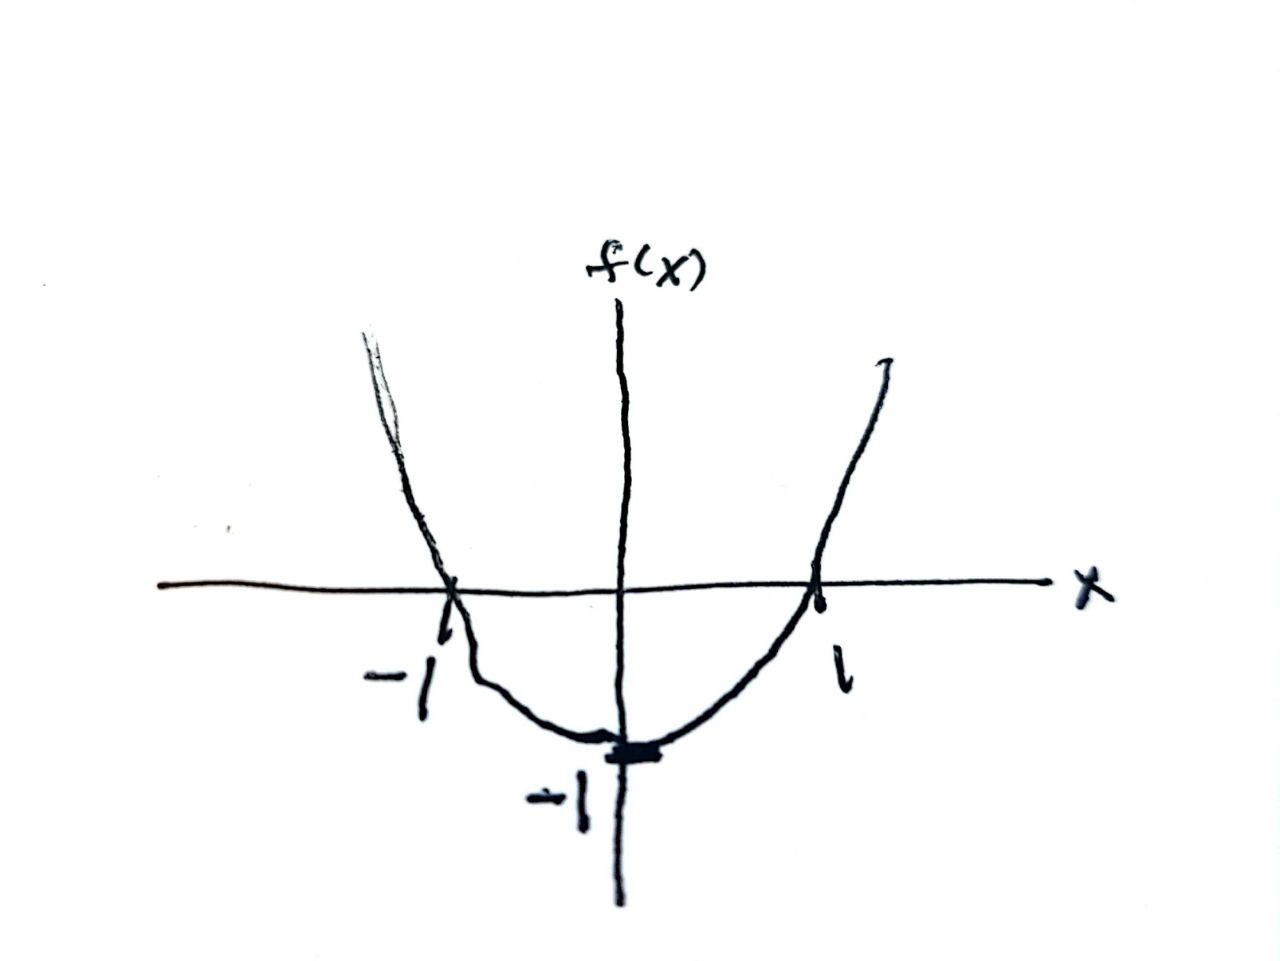
\includegraphics[width=0.6\textwidth]{4.jpg}
    \label{fig:4-jpg}
\end{figure}


(b) We have $G(f) = V\left( x_{n+1} - f(x_1, \ldots, x_n) \right) \subset 
\mathbb{A}^{n+1}$ where $x_{n+1} - f\left( x_1,\ldots,x_n \right) $ is
polynomial, since it is the difference of two polnomials since $f$ is
a polynomial.\\
\linebreak
(c) We define the morphisms
$\varphi  \colon X \to G(f)$ by
$\varphi (a_1, \ldots, a_n) = \left( a_1, \ldots, a_n, f(a_1, \ldots, a_n)
\right) $ and
$pr_X  \colon G(f) \to X$ by $pr_X \left( a_1, \ldots, a_{n+1} \right) 
= \left( a_1, \ldots, a_n \right) $. Clearly,
$pr_X \circ \varphi = \mathbbm{1}_X$ and $\varphi \circ pr_X
= \mathbbm{1}_{G_f}$. Furthermore, $\varphi$ is a morphism since
$\varphi (P) = \left(x_1 (P), x_2 (P), \ldots, x_n(P) ,f(P) \right) $
for all $P \in X$, and 
$x_1, \ldots, x_n, f \in k\left[ x_1, \ldots, x_n \right] $.
The projection map is also a morphism by the first example on lecture note 8.
Thus $G(f)$ is isomorphic to $X$.












































\end{document}
